\documentclass[sigconf,screen,review]{acmart}

\setcopyright{none}
\settopmatter{printacmref=false, printccs=false, printfolios=true}
\renewcommand\footnotetextcopyrightpermission[1]{}
\pagestyle{plain}

\usepackage{booktabs}
\usepackage{array}
\usepackage{enumitem}
\usepackage{xcolor}
\usepackage{graphicx}
\usepackage{balance}

\setlist[itemize]{leftmargin=1.2em}
\setlist[enumerate]{leftmargin=1.4em}
\renewcommand{\arraystretch}{1.08}

\title{Weekly Report}
\subtitle{Week of June 30, 2026}

\begin{document}

\maketitle

\section{Mechanism 1}

\subsection{Implemented Mechanism}

Mechanism~1 targets the cache/DRAM data path.  The implementation was cleaned
up to keep only the simple batching opportunities that match the simulator's
memory hierarchy:

\begin{itemize}
  \item \textbf{L2 directory lookup batching.}  Directory lookup selects one
  cache set and scans multiple ways.  Mechanism~1 batches requests that can
  reuse this set/way lookup work, reducing repeated lookup overhead when
  multiple requests arrive close together.
  \item \textbf{DRAM access-unit coalescing.}  A 64B L2 miss is handled by the
  DRAM timing model at a 128B aligned access unit.  Two adjacent 64B cache
  lines that fall into the same 128B access unit can therefore be coalesced
  before entering DRAM timing.
\end{itemize}

The code was simplified by removing extra knobs that were not needed for the
core experiment.  The intended conclusion is narrow: Mechanism~1 should reduce
work on the L2/DRAM path when spatially adjacent requests or same-set
directory probes appear close together.

\subsection{Current Observation}

The earlier M1 runs showed that some local path metrics improved, including
L1V and L2 latency components, but the end-to-end runtime speedup was small or
inconsistent.  This suggests that Mechanism~1 is active but often not on the
dominant critical path.  In several workloads, removing a local memory-system
bottleneck exposes another downstream bottleneck such as remote network
service, MSHR waiting, or synchronization.

\section{Mechanism 2}

\subsection{Implemented Mechanism}

Mechanism~2 implements a requester-side RDMA batch queue.  Its purpose is to
batch nearby remote requests before they are injected into the remote access
path.  This is complementary to Mechanism~1: M1 targets the L2/DRAM side,
whereas M2 targets the requester-side remote access path before the request is
sent across the wafer network.

The run infrastructure now supports four experiment modes:
\begin{itemize}
  \item \texttt{baseline}
  \item \texttt{m1}
  \item \texttt{m2}
  \item \texttt{m1\_m2}
\end{itemize}

This makes it possible to run a direct ablation study with the same benchmark,
sampling, and maximum-workgroup settings.

\subsection{Current Observation}

The available M1/M2 results still do not show a large end-to-end improvement.
At this point the best interpretation is not that the mechanisms are inactive,
but that the optimized datapaths are not always the limiting path.  The next
step is therefore to combine ablation experiments with critical-path tracing:
for each workload, determine whether the dominant remaining time is address
translation, L1V local work, L2/DRAM service, RDMA/network transfer, or
workload synchronization.

\section{M1/M2 Experimental Results}

\subsection{Four-Way Ablation}

The four-way ablation run compares baseline, M1, M2, and M1+M2 using the same
\texttt{sample\_all\_w512\_g512} configuration.  Table~\ref{tab:m1m2-ablation-all}
lists all benchmark entries from the June 29 all-mechanisms ablation run.
Blank cells indicate comparisons where usable metrics were not available.

Only seven workloads have all four mechanism variants and also reached the
max-workgroup limit in every variant.  On this valid subset, the geometric-mean
speedups are:

\begin{itemize}
  \item M1: 0.999$\times$ ($-0.06\%$)
  \item M2: 1.012$\times$ ($+1.19\%$)
  \item M1+M2: 1.004$\times$ ($+0.36\%$)
\end{itemize}

Figure~\ref{fig:m1m2-ablation} visualizes the available entries from the same
June 29 result directory as simulation-time improvement over baseline.  The main
signal is that M2 helps FloydWarshall, while PageRank is a negative case for
the combined mechanism.  Most other valid workloads are close to neutral.  The
larger speedups shown by FIR, matrix multiplication, simple convolution, and
SpMV in Table~\ref{tab:m1m2-ablation-all} are not included in the aggregate
because they did not reach the max-workgroup limit.

\begin{table*}[t]
  \centering
  \caption{All benchmark entries in the four-way M1/M2 ablation run.  Values
  are speedup over baseline.  Blank cells indicate unavailable metrics.}
  \label{tab:m1m2-ablation-all}
  \scriptsize
  \begin{tabular}{lccc}
    \toprule
    Workload & M1 & M2 & M1+M2 \\
    \midrule
    AES & & & \\
    BitonicSort & 1.012$\times$ & 1.000$\times$ & 1.012$\times$ \\
    FastWalshTransform & 1.018$\times$ & 1.002$\times$ & 1.022$\times$ \\
    FFT & 1.004$\times$ & 1.000$\times$ & 1.004$\times$ \\
    FIR & 5.673$\times$ & & 5.766$\times$ \\
    FloydWarshall & 0.994$\times$ & 1.068$\times$ & 1.069$\times$ \\
    Im2Col & 1.006$\times$ & 1.005$\times$ & 1.004$\times$ \\
    KMeans & & & \\
    MatrixMultiplication & 1.377$\times$ & 1.384$\times$ & 1.403$\times$ \\
    MatrixTranspose & & & 1.000$\times$ \\
    PageRank & 0.963$\times$ & 1.011$\times$ & 0.920$\times$ \\
    ReLU & 1.000$\times$ & 1.000$\times$ & 1.000$\times$ \\
    ResNet & & 1.000$\times$ & \\
    SimpleConvolution & 1.440$\times$ & 0.999$\times$ & 1.360$\times$ \\
    SpMV & & 1.068$\times$ & 0.989$\times$ \\
    \bottomrule
  \end{tabular}
\end{table*}

\begin{figure*}[t]
  \centering
  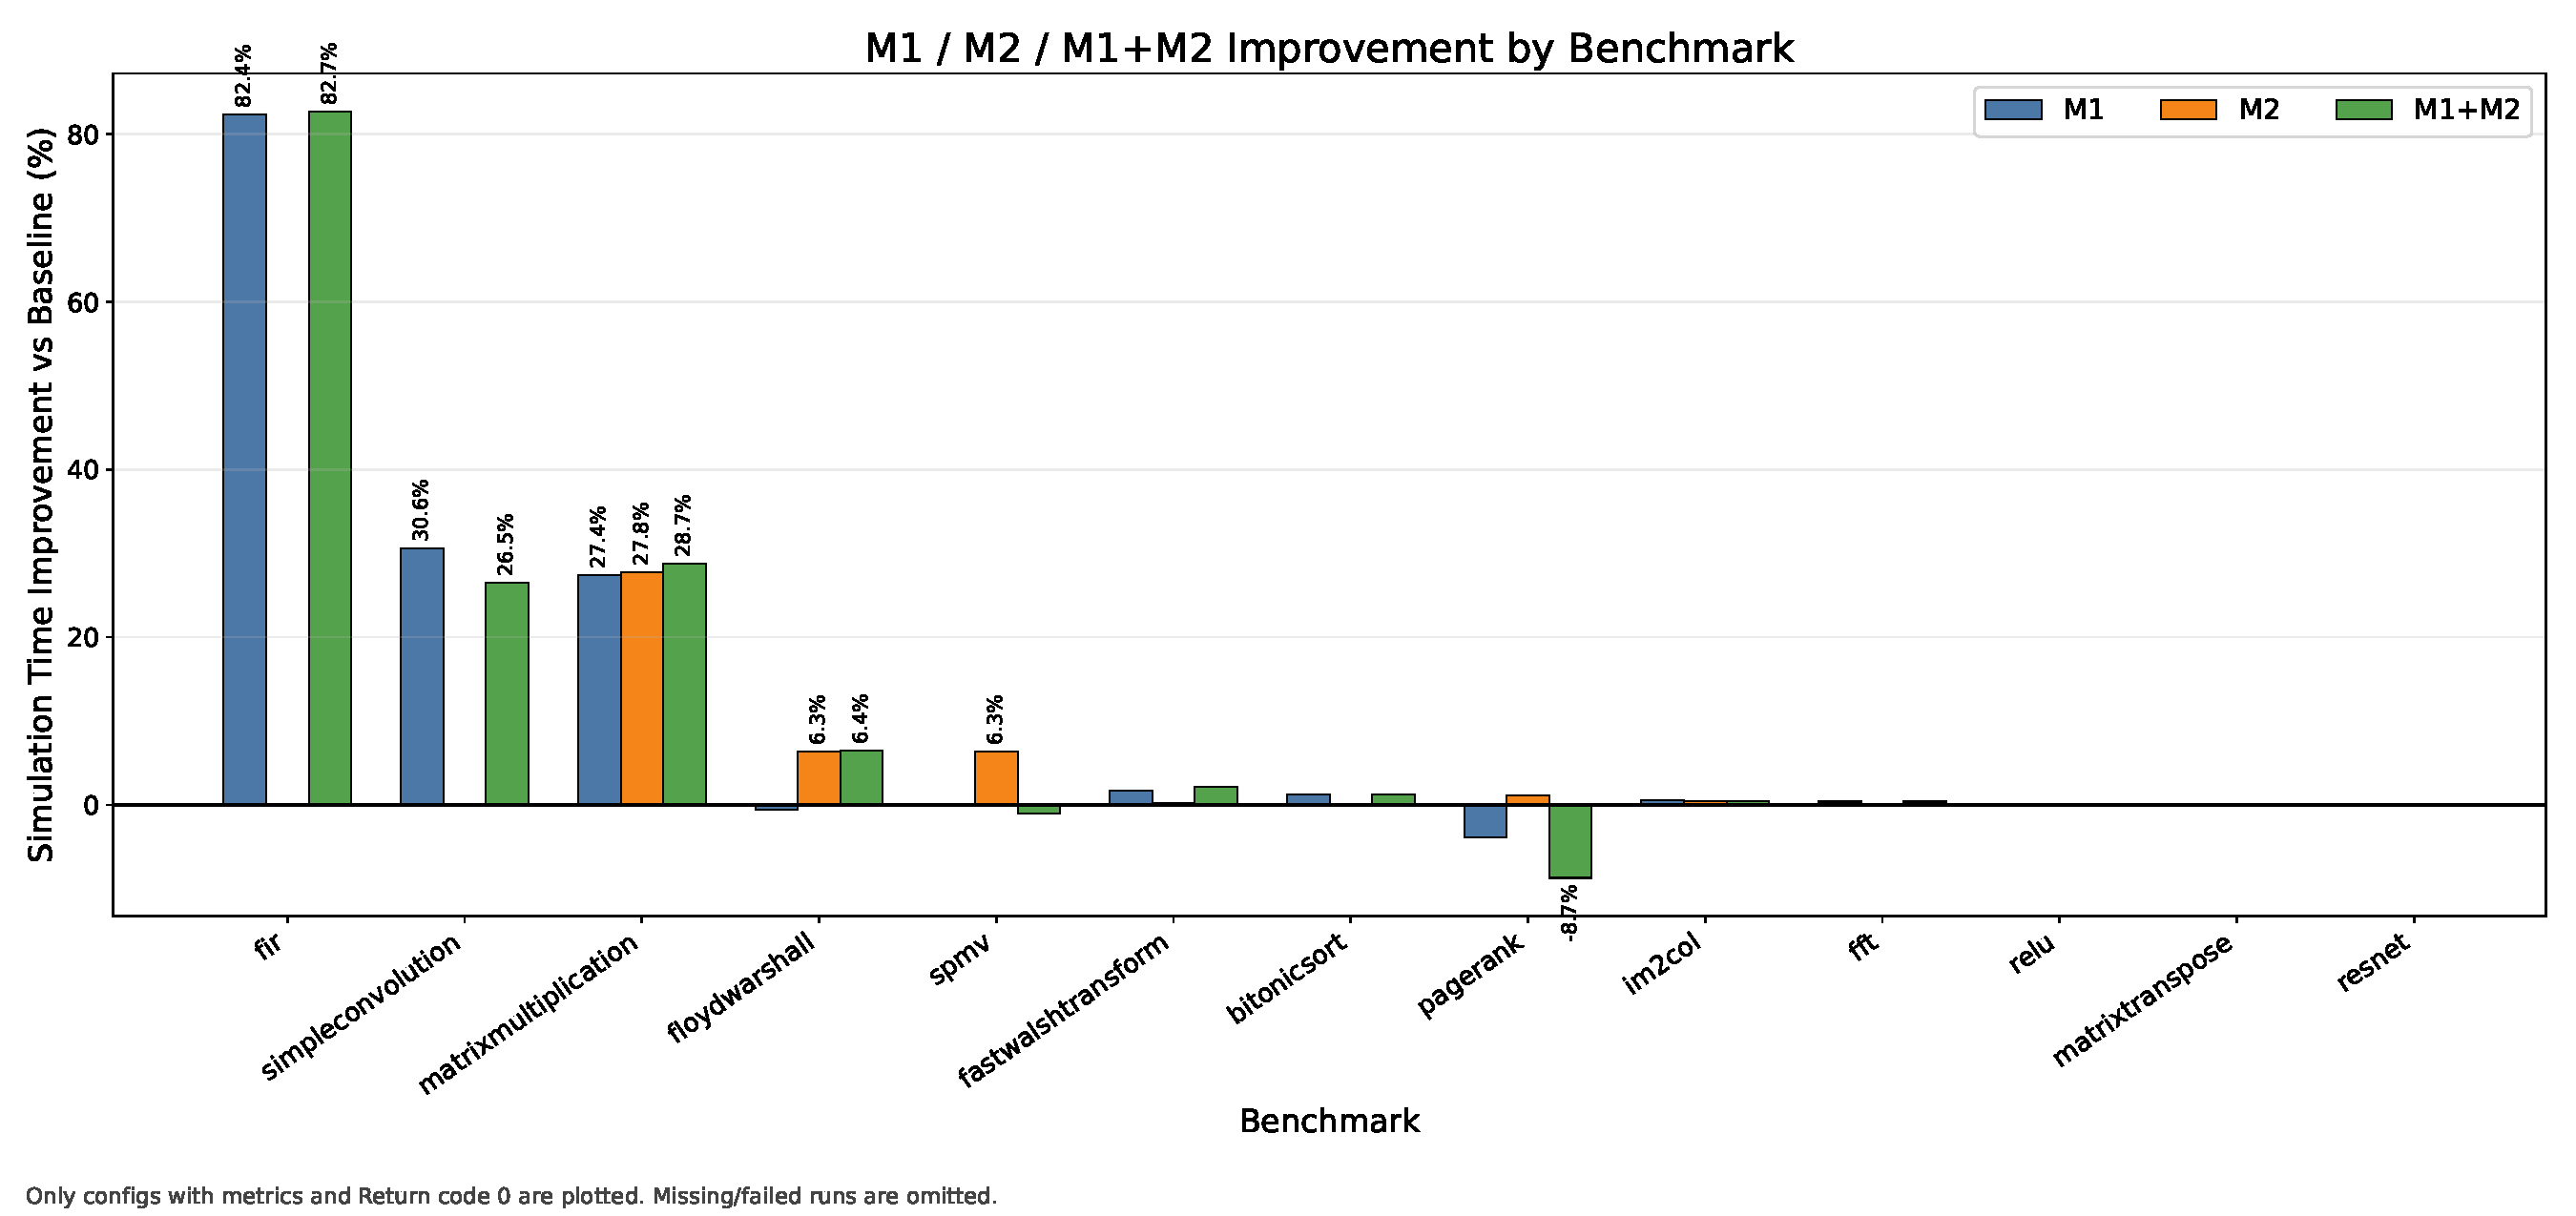
\includegraphics[width=0.95\textwidth]{figures/m1_m2_ablation_speedup.pdf}
  \caption{M1/M2 four-way ablation from the June 29 all-mechanisms run.  Bars
  show simulation time improvement relative to baseline.}
  \label{fig:m1m2-ablation}
\end{figure*}

\subsection{Baseline vs. M1+M2 From the Ablation Run}

Table~\ref{tab:m1m2-final} also uses the June 29 all-mechanisms ablation run.
It expands the combined mechanism comparison by listing the baseline and M1+M2
\texttt{Driver.total\_time} values used to compute speedup.  On the
seven-workload valid subset, the
geometric-mean M1+M2 speedup is 1.004$\times$ (+0.36\%).

\begin{table*}[t]
  \centering
  \caption{Baseline vs. M1+M2 results from the June 29 all-mechanisms ablation
  run.  Time is
  \texttt{Driver.total\_time}; speedup is baseline time divided by M1+M2 time.}
  \label{tab:m1m2-final}
  \scriptsize
  \begin{tabular}{lrrr}
    \toprule
    Workload & Baseline time ($\mu$s) & M1+M2 time ($\mu$s) & Speedup \\
    \midrule
    AES & & & \\
    BitonicSort & 84.257 & 83.237 & 1.012$\times$ \\
    FastWalshTransform & 366.504 & 358.784 & 1.022$\times$ \\
    FFT & 967.290 & 963.588 & 1.004$\times$ \\
    FIR & 1151.002 & 199.616 & 5.766$\times$ \\
    FloydWarshall & 93.106 & 87.110 & 1.069$\times$ \\
    Im2Col & 116.393 & 115.891 & 1.004$\times$ \\
    KMeans & & & \\
    MatrixMultiplication & 10085.898 & 7187.314 & 1.403$\times$ \\
    MatrixTranspose & 27154.072 & 27148.151 & 1.000$\times$ \\
    PageRank & 11351.973 & 12341.267 & 0.920$\times$ \\
    ReLU & 83.072 & 83.031 & 1.000$\times$ \\
    ResNet & 1823.925 & & \\
    SimpleConvolution & 61.012 & 44.853 & 1.360$\times$ \\
    SpMV & 139115.230 & 140599.579 & 0.989$\times$ \\
    \midrule
    Valid geomean & & & 1.004$\times$ \\
    \bottomrule
  \end{tabular}
\end{table*}

\subsection{Interpretation}

The current evidence is mixed.  M1/M2 can reduce end-to-end time in selected
workloads, but the average effect is still small.  This is consistent with the
critical-path traces: even when a mechanism reduces part of the L2/DRAM or
RDMA path, the application can remain limited by another path such as L1V
MSHR waiting, remote network imbalance, synchronization, or address
translation.  The mechanism result should therefore be presented as a
promising but not yet sufficient optimization, and the next experiment should
connect each speedup or slowdown to the traced critical path.

\section{Experiment Infrastructure}

\subsection{Run Script Consolidation}

The Python experiment flow was consolidated into a single runner script.  The
script now supports the following core features:

\begin{itemize}
  \item mechanism selection through \texttt{--mechanisms}
  (\texttt{baseline}, \texttt{m1}, \texttt{m2}, \texttt{m1\_m2}, or
  \texttt{all});
  \item traditional benchmark presets and \texttt{sample\_all} configuration
  selection;
  \item Photon sampling flags;
  \item build-before-run behavior;
  \item \texttt{--max-workers} for concurrent workload control;
  \item memory-gated launch using Linux \texttt{MemAvailable};
  \item direct memory-path trace flags for critical-path studies.
\end{itemize}

The PTCL-related flow was removed from the main script so that the current
experiments focus only on baseline, M1, M2, and M1+M2.

\subsection{Scheduling Lessons}

The memory-gated scheduler works as intended: it fills the queue up to the
worker cap and then launches another benchmark only after one finishes and the
available memory threshold is satisfied.  However, full request-level tracing
can produce very large files.  The most recent remote-only baseline trace used
about 99GB of disk space.  The largest files were the raw hop traces for SpMV
(43GB), matrix transpose (33GB), and PageRank (11GB).  This indicates that a
future trace mode should avoid writing full hop-level raw traces unless they
are specifically needed.

\section{Critical-Path and Remote-Network Trace}

\subsection{Streaming Memory-Path Trace}

The previous memory-path tracer stored completed request records and raw rows
in RAM until the end of the run.  This caused remote-heavy workloads such as
SpMV to be killed when \texttt{--trace-memory-path-max-records=0} was used.

This week I added a streaming mode:

\begin{itemize}
  \item \texttt{--trace-memory-path-stream} writes memory-path raw rows,
  L1V-path summaries, and L1V-hop rows directly to output files;
  \item completed request records are released after they are written;
  \item \texttt{--trace-memory-path-remote-only} can be combined with streaming
  so that warmup and record limits apply only to remote L1V paths;
  \item \texttt{--trace-memory-path-max-records=0} now remains useful for full
  remote-path collection without linearly growing RAM usage.
\end{itemize}

The streaming path was validated with a unit test that constructs a synthetic
remote L1V request, confirms that the trace files are written, and checks that
the completed record is released from the in-memory record map.

\subsection{Remote-Only Baseline Trace}

I ran a baseline remote-only streaming trace over the traditional benchmarks.
The result is not a clean performance run: several remote-heavy workloads were
killed or externally stopped before final metrics were written.  However, the
streamed records are still useful for motivating the remote datapath and
network-imbalance problem because they are written before the process exits.

Figure~\ref{fig:remote-network-motivation} summarizes the remote-heavy
benchmarks.  Zero-remote benchmarks are omitted.

\begin{figure*}[t]
  \centering
  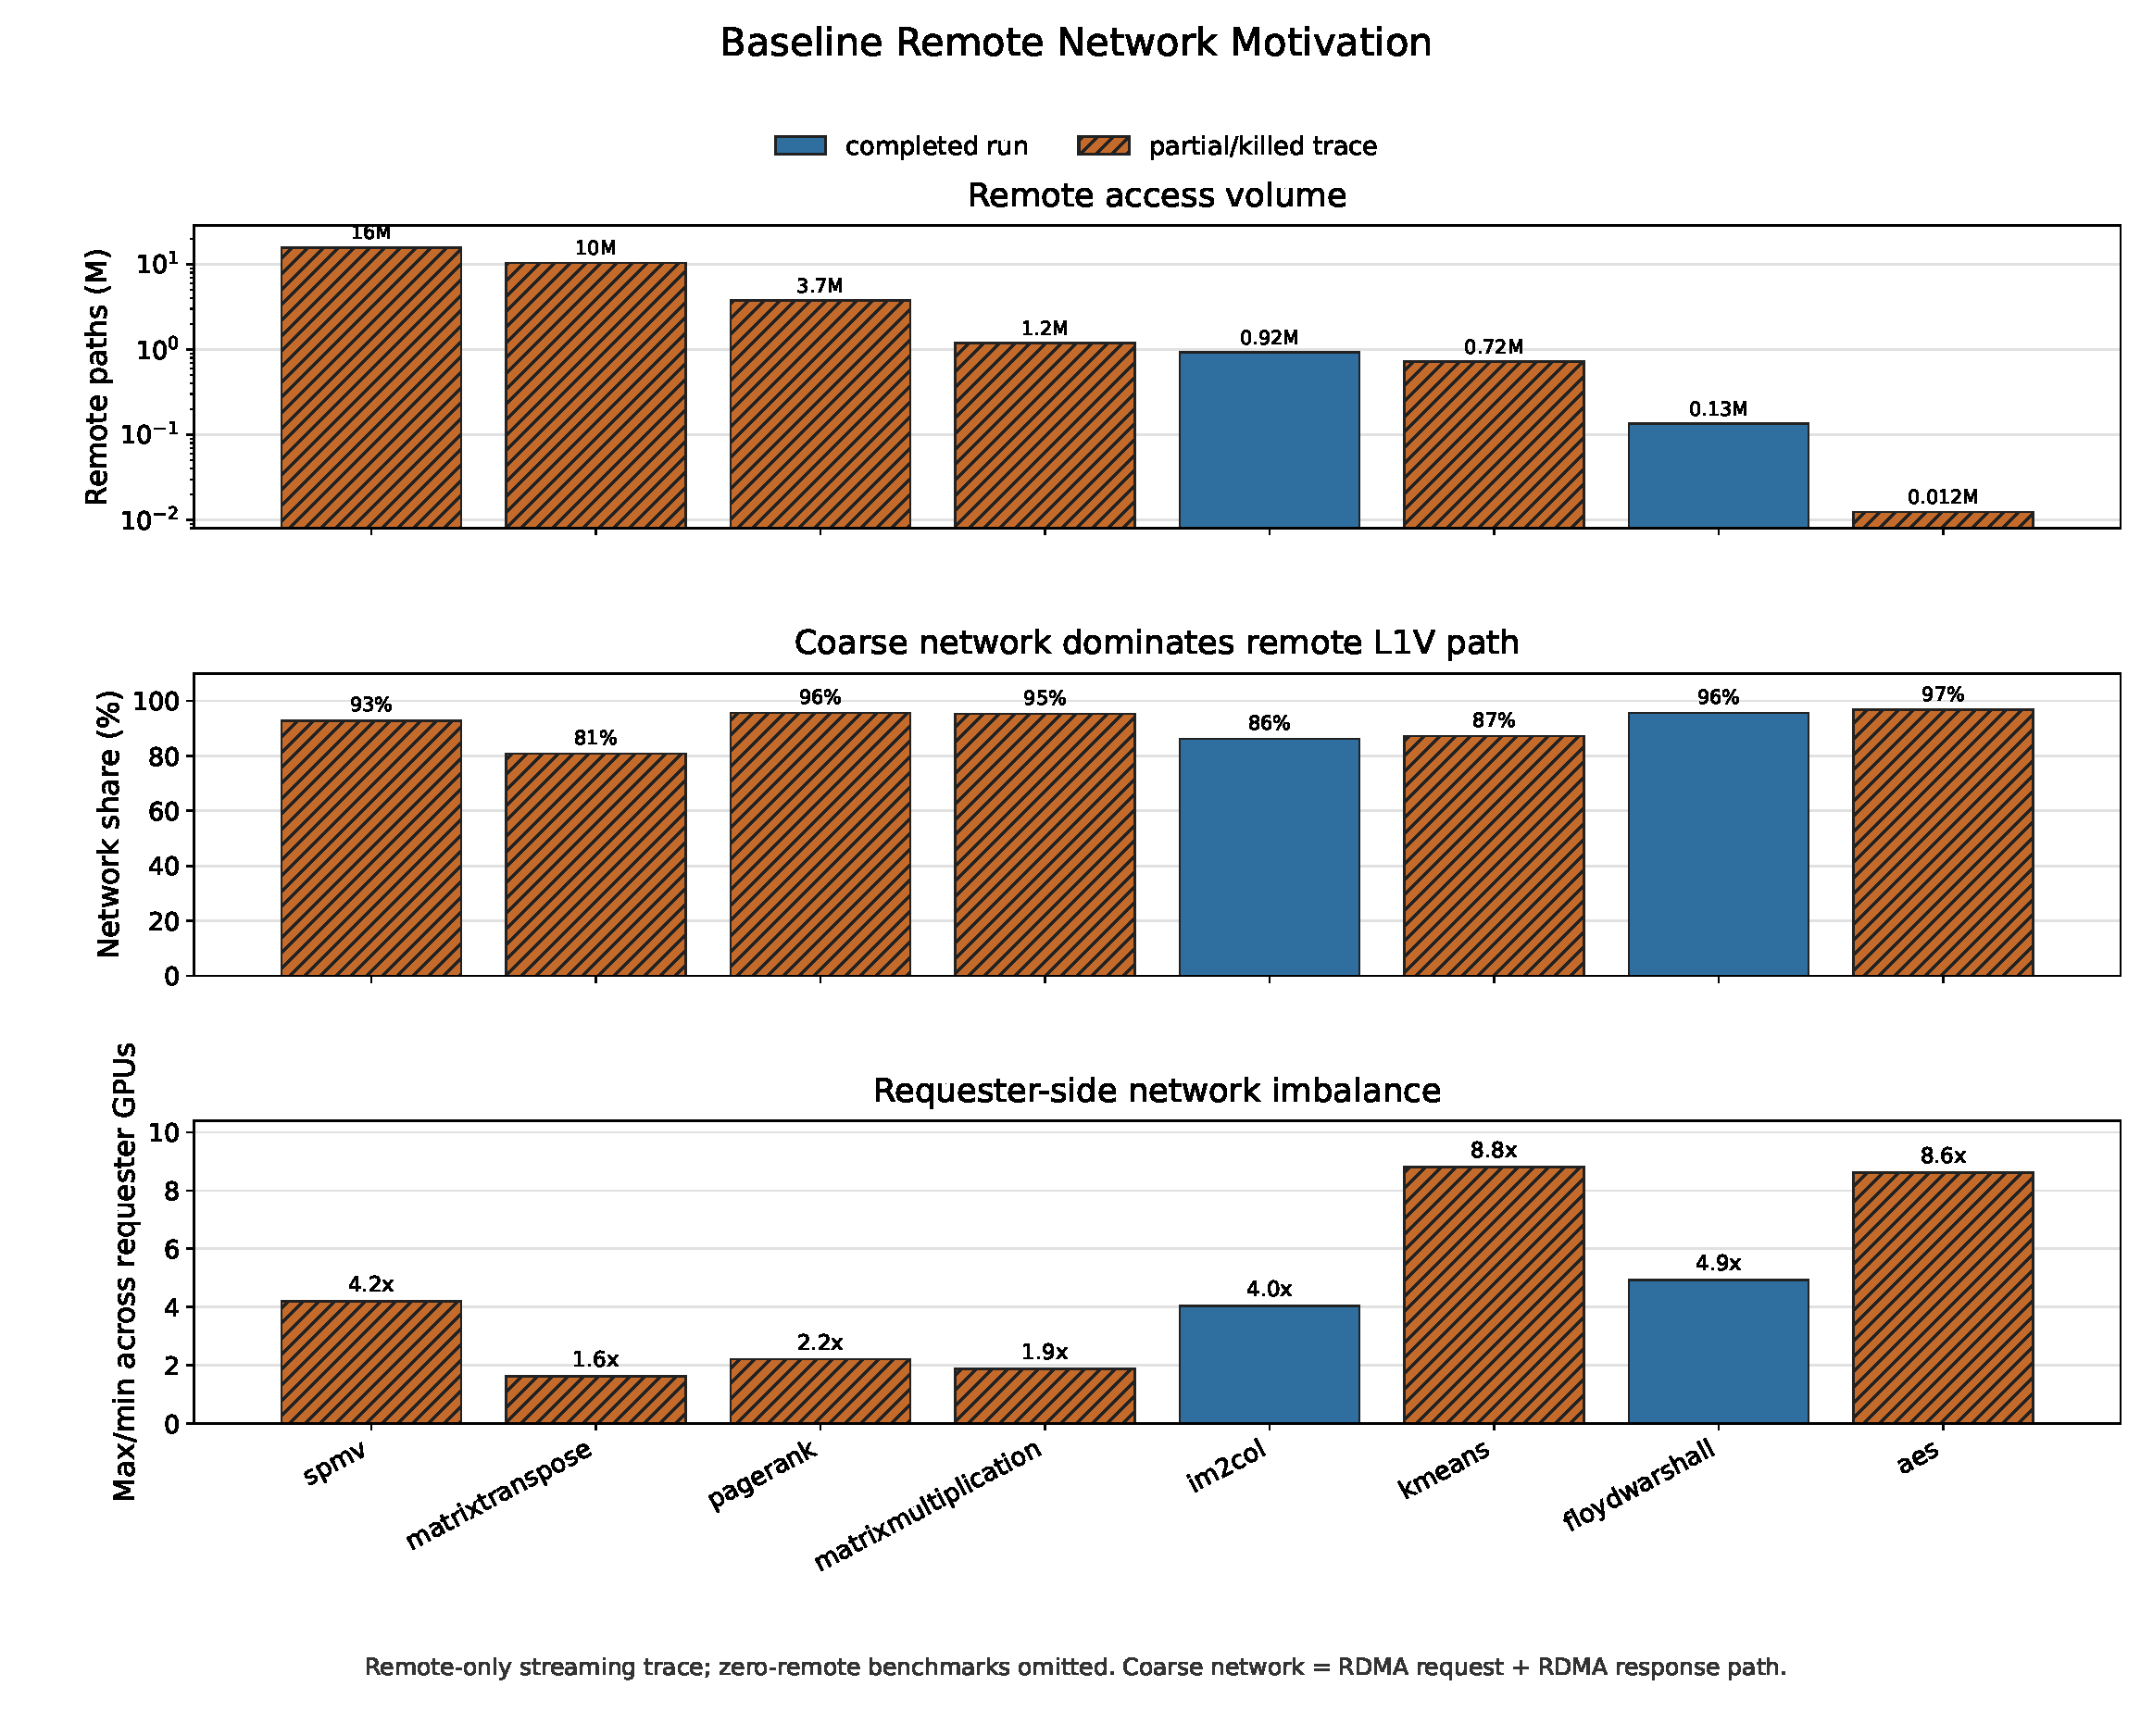
\includegraphics[width=0.98\textwidth]{figures/baseline_remote_network_motivation.pdf}
  \caption{Baseline remote-network motivation from the remote-only streaming
  trace.  The top panel shows remote L1V path count.  The middle panel shows
  the fraction of the remote L1V path explained by coarse network/RDMA latency
  (RDMA request plus RDMA response path).  The bottom panel shows requester GPU
  imbalance as the max/min ratio of average coarse network latency across
  requester GPUs.}
  \label{fig:remote-network-motivation}
\end{figure*}

\begin{table*}[t]
  \centering
  \caption{Remote-only baseline trace summary.  ``Network share'' uses the
  coarse RDMA request+response path, not the cumulative fine-grained flit-stage
  sum.}
  \label{tab:remote-summary}
  \begin{tabular}{lrrrr}
    \toprule
    Workload & Remote paths & Avg coarse network & Network share & GPU max/min \\
    & (M) & (ns) & (\%) & \\
    \midrule
    SpMV & 15.78 & 302.6 & 92.7 & 4.20$\times$ \\
    MatrixTranspose & 10.42 & 364.7 & 80.8 & 1.61$\times$ \\
    PageRank & 3.74 & 369.5 & 95.6 & 2.21$\times$ \\
    MatrixMultiplication & 1.19 & 1213.4 & 95.3 & 1.87$\times$ \\
    Im2Col & 0.92 & 257.2 & 86.2 & 4.03$\times$ \\
    KMeans & 0.72 & 525.5 & 87.2 & 8.80$\times$ \\
    FloydWarshall & 0.13 & 702.6 & 95.6 & 4.93$\times$ \\
    AES & 0.01 & 532.2 & 96.7 & 8.61$\times$ \\
    \bottomrule
  \end{tabular}
\end{table*}

\section{Main Takeaways}

\begin{enumerate}
  \item \textbf{Remote-heavy workloads exist and are measurable.}  SpMV,
  matrix transpose, PageRank, matrix multiplication, Im2Col, KMeans, and
  FloydWarshall all show substantial remote L1V path activity.

  \item \textbf{The remote L1V path is network dominated.}  In the coarse
  RDMA-path view, network/RDMA accounts for roughly 81--97\% of the remote
  L1V path in the remote-heavy workloads.

  \item \textbf{Requester GPU imbalance is large.}  The max/min ratio of
  average requester-side network latency ranges from 1.6$\times$ to
  8.8$\times$.  This supports using network imbalance as a motivation for
  requester-side batching or scheduling.

  \item \textbf{Zero-remote workloads should not be expected to benefit from
  M2.}  BitonicSort, FFT, FIR, ReLU, and SimpleConvolution have zero remote
  paths in this trace window, so remote-access batching is unlikely to affect
  their end-to-end runtime.

  \item \textbf{Full hop-level tracing is too expensive for routine sweeps.}
  Streaming fixes the RAM problem, but the raw hop files are still very large.
  A summary-only mode is needed for overnight sweeps.
\end{enumerate}

\section{Next Steps}

\begin{itemize}
  \item Add a \texttt{summary-only} or \texttt{no-hop-raw} memory-path trace
  mode.  This should keep per-GPU and per-GPU-pair aggregate counters while
  avoiding tens of GB of hop-level raw trace output.

  \item Re-run the traditional benchmark ablation with
  \texttt{baseline}, \texttt{m1}, \texttt{m2}, and \texttt{m1\_m2}.  Use the
  same \texttt{--max-wg}, Photon sampling settings, and worker count for all
  mechanisms.

  \item For remote-heavy workloads, collect both end-to-end metrics and
  summary-only critical-path data.  The goal is to determine whether M1/M2
  reduce network/RDMA path time, L2/DRAM service time, or only local cache
  latency.

  \item For workloads without speedup, identify whether the remaining critical
  path is synchronization, address translation, local L1V/L2 behavior, or
  network imbalance.
\end{itemize}

\section{Artifacts}

The main artifacts produced this week are:

\begin{itemize}
  \item consolidated experiment runner;
  \item M1/M2 mechanism toggles and ablation flow;
  \item remote-only memory-path tracing;
  \item streaming memory-path trace mode;
  \item coarse-network and requester-GPU imbalance summary CSVs;
  \item remote-network motivation figure used in this report.
\end{itemize}

\balance

\end{document}
